%%%%%%%%%%% Aquí va la solución al problema 4.
\newpage
\textbf{\textcolor{MidnightBlue}{4.}} Considera el algoritmo 1,
que calcula una $\Delta + 1$ coloración, donde $\Delta$ es el
grado máximo en la gráfica. Muestra una gráfica $G$ con al menos
10 vértices y una asignación de IDs, donde el algoritmo coloree
todos los procesos (el primer momento en el que todas las variables
$c$ son distintas de $\bot$) en tiempo $diam(G)$. Muestra otra
asignación de IDs para las que el algoritmo coloree en tiempo a los
más $diam(G)/2$.

\begin{figure}[ht]
        \begin{center}
                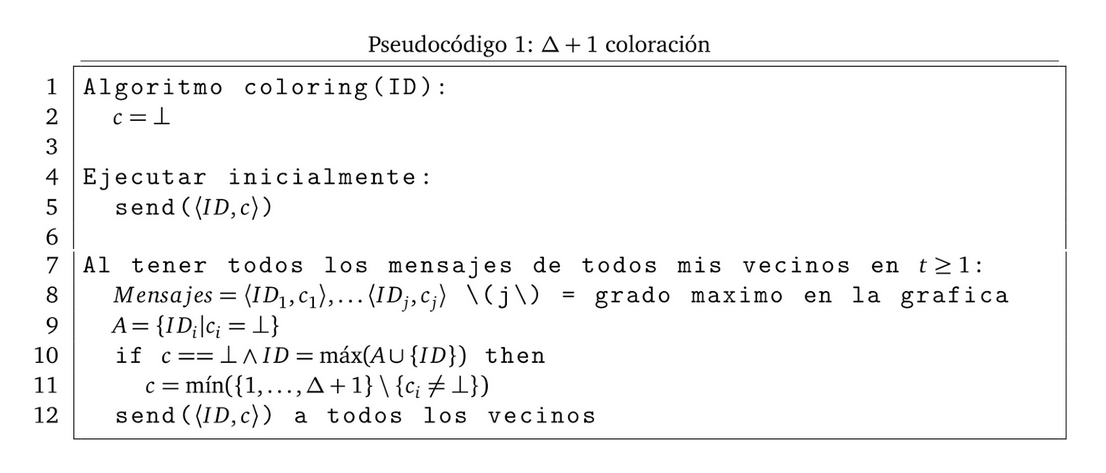
\includegraphics[width=15cm]{AlgoritmoP5.png}
        \end{center}
\end{figure}

$\rhd$ Para este problema dividamos la solución en $3$ respectivas
soluciones:                                                             \newline

\hspace*{0.5cm} \textbf{\textcolor{blue}{1}}. Mostrar una ejecución
en tiempo \code{diam($G$)}, con $G$ una gráfica tal que $|V_G| = 10$.

\begin{figure}[ht!]
     \centering
     \begin{tikzpicture}
        \begin{scope}
           % Fig exterior:
           \node(0) [vertex, label=180:$p_0$] at (-2, 0)       {};
           \node(1) [vertex, label=180:$p_1$] at (2,  0)       {};
           \node(2) [vertex, label=180:$p_2$] at (3.24, 3.81)  {};
           \node(3) [vertex, label=180:$p_3$] at (0, 6)        {};
           \node(4) [vertex, label=180:$p_2$] at (-3.24, 3.81) {};
           % Fig interior:
           
           
           \node (L) at (-5,5){$G$};
        \end{scope}
     \end{tikzpicture}
\caption{Gŕagica $G$.}
\label{fig:fam1}
\end{figure}

\hfill $\lhd$
